\section{Natural Language Understanding}
Natural Language Understanding (NLU) systems process human generated text (or speech) at a deep semantic level and encode the meaning
of the processed inputs. Several concrete tasks have been defined within the field on Computational Linguistics (CL) to evaluate the encoded meaning representations.
In the case of Semantic Parsing, the output is a logical form that can be queried against a knowledge base of facts to compute its truth value. Textual Entailment refers to the 
problem of identifying whether the truth of some text provided as a hypothesis follows from that of another text provided as a premise. Sentiment Analysis is the process of 
automatically categorizing the opinions expressed in the inputs towards specific targets. All these tasks require encoding the semantics of the input in a way that is
at least good enough to perform well at the given task, with the inherent assumption that an improvement in the task performance correlates with an improvement in the
quality of the semantic representation or in other words, the understanding capability of the computational system.
% TODO: Improve the following statement and uncomment it.
%Each task defines a restricted set of linguistic aspects that can be taught to a computational system, and are easy enough to automatically evaluate
%on unseen examples, but are complex enough for the representation techniques to be applicable to understanding the unrestricted set.

A generic NLU system can thus be succinctly described using the following two equations.
\begin{align}
 \mathbf{e} &= \mathtt{encode}(\mathbf{I}) \label{eq:generic_encoding}\\
 \mathbf{o} &= \mathtt{predict}(\mathbf{e}) \label{eq:generic_prediction}
\end{align}
where $\mathbf{I}$ is the set of textual inputs to the NLU system. 
%TODO: Concrete examples of systems that fit in this paradigm.
For example, $\mathbf{I}$  are single sentences in Sentiment Analysis and pairs of sentences in Textual Entailment. $\textbf{e}$ are intermediate 
encoded semantic representations of the inputs (which may or may not be task specific), and $\mathbf{o}$ are the final task specific predictions. For example, in Sentiment Analysis or Textual Entailment, 
$\mathbf{o}$ are categorical labels indicating the sentiment or entailment respectively, and in the case of Semantic Parsing, they are structured outputs or parses. In older feature-rich methods for NLU, 
Equation~\ref{eq:generic_encoding} is a mapping of the inputs to a hand designed feature space, typically containing patterns over word classes based on part-of-speech \cite{corley2005measuring} or Wordnet synsets \cite{moldovan2001logic} 
shallow linguistic features like dependencies \cite{bos2005recognising} or named entities \cite{tatu2005semantic}. In such systems,
the modeling emphasis was more on the prediction component, and the encoding component did not involve any learning. More recent systems \cite{weston2014memory,hermann2015teaching,Sukhbaatar2015EndToEndMN,Xiong2016DynamicMN} 
use representation learning techniques to also learn the parameters of the
$\mathtt{encode}$ function, and typically this is done jointly with learning the parameters of the $\mathtt{predict}$ function.

\section{Need for External Knowledge}
\label{sec:intro_external_knowledge}
\subsection{Background Knowledge}
An issue with the formulation of the problem in Equation~\ref{eq:generic_encoding} and Equation~\ref{eq:generic_prediction} is that they are missing a key input: \textbf{background knowledge}. 
Since human language is aimed at other humans who share 
the same background knowledge, a lot of information is often not explicitly stated
for the sake of brevity. The implicit knowledge required to understand language varies 
from simple commonsense in the case of basic conversations, to complex principles that link 
concepts in more esoteric communications. Consider an example of the former in solving the 
textual entailment problem given the following premise, and a candidate hypothesis:
\begin{itemize}
 \item \textbf{Premise:} \textit{Children and parents are splashing water at the pool.}
 \item \textbf{Hypothesis} \textit{Families are playing outside.}
\end{itemize}
The knowledge a human uses to correctly predict that the hypothesis can be inferred from the 
premise is that \textit{children and parents} typically form \textit{families}, \textit{splashing water} 
is a kind of \textit{playing}, and a \textit{pool} is expected to be \textit{outside}. An entailment model trained on texts like the
ones shown above, with just the sentences as inputs, will not have access to the background knowledge that humans possess. Such a model
will at best memorize co-occurrence patterns in the input words. Using pre-trained vectors to represent input words provides additional
knowledge to the model in the form of co-occurrence statistics obtained from large corpora. However, it is unclear whether distributional
information alone can substitute the kind of knowledge described above. Fortunately, background knowledge is encoded to some extent in machine readable
ontologies and knowledge bases. In this thesis, we will show how such background knowledge can be leveraged to improve lexical representations, and used
in conjunction with distributional models to obtain better input representations for NLU systems.

\subsection{Contextual Knowledge}
A second issue with the generic NLU formulation is that it does not account for the context in which the input utterance occurs. Typically, context
includes the circumstances that form the setting for the input utterances to be fully understood, and hence it significantly contributes to the meaning of the
inputs. In this thesis, we will refer to this additional information as \textbf{contextual knowledge}. Unlike background knowledge, this is not implicit in the
text being read. However, reasoning in the presence of contextual knowledge still poses significant challenges. An automated reading comprehension system that processes this additional information
is expected to encode it in a way such that the relevant parts of the information can later be retrieved when predictions are being made about the input sentences.
Several such tasks have been proposed in the past. Examples include \cite{hill2015goldilocks,richardson2013mctest,penas2013qa4mre,breck2001looking}, and necessitate varying levels of reasoning complexity. It has generally been established
that training automated systems to reason given context is extremely difficult unless one sets constraints on the task such as simplifying the language or controlling the scope of
context.

Figure~\ref{fig:babi_example} shows an example from the bAbI dataset \citep{weston2015towards}, which is a collection of artificially generated toy tasks. The first six sentences in the example
form the context, and the final line is a question followed by the answer and pointers to the relevant sentences in the context. A QA system is expected to learn to find the appropriate context
given the question and answer it correctly.
\begin{figure}
\begin{center}
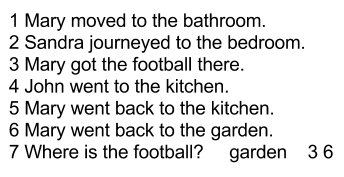
\includegraphics[width=3in]{figures/bAbI_example.png}
\caption{Example of an artificial task requiring reasoning over context, part of the bAbI dataset}
\label{fig:babi_example}
\end{center}
\end{figure}

Figure~\ref{fig:science_qa_example} shows a relatively more difficult QA example from Aristo science question answering dataset \citep{clark2015elementary}. Simple techniques such as measuring lexical overlap do not
work well for this task because all four options have significant overlap with the sentences in context. As we show in Chapter~\ref{chapter:memnet_qa}, this task requires modeling complex entailment to be able to match the information present in the context with that in the question and
option pairs.
\begin{figure}
\begin{center}
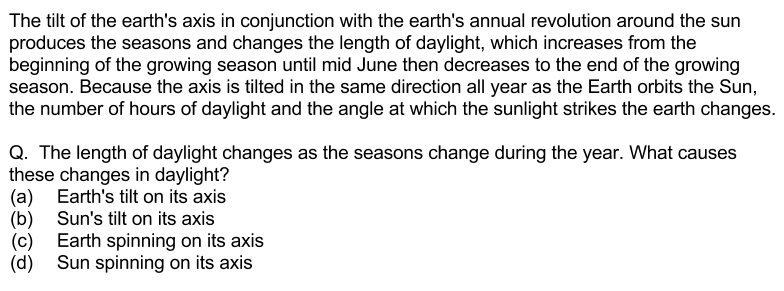
\includegraphics[width=6in]{figures/science_qa_example.png}
\caption{Snippet from a science textbook followed by a question}
\label{fig:science_qa_example}
\end{center}
\end{figure}


\section{Incorporating External Knowledge}
Clearly, we need to incorporate external knowledge of both kinds described above, into our NLU systems.
Without background knowledge, the NLU systems will merely memorize specific patterns seen in the training data
and cannot generalize to unseen test cases. Without contextual knowledge, they cannot reason over large spans of text in reading comprehension tasks.
We thus modify our NLU equations as follows.
\begin{align}
 \mathbf{e} &= \mathtt{encode\_with\_knowledge}(\mathbf{I}, \mathbf{K}_e) \label{eq:encoding_with_knowledge}\\
 \mathbf{e}_{K_p} &= \mathtt{encode}(\mathbf{K}_p) \\ \label{eq:knowledge_encoding}
 \mathbf{o} &= \mathtt{predict\_with\_knowledge}(\mathbf{e}, \mathbf{e}_{K_p}) \label{eq:prediction_with_knowledge}
\end{align}
where $\mathbf{K}_e$ and $\mathbf{K}_p$ represent the knowledge required for encoding and prediction respectively. 
They come from different sources and augment the inputs in different ways as described below.

\subsection{Better encoding with background knowledge}
$\mathbf{K}_e$ is additional knowledge used to better compose the units in input text. Particularly, this allows for
obtaining input encoding that respects the selectional restrictions of the units being composed.
Examples of $\mathbf{K}_e$ include hypernym trees from WordNet for
incorporating sense and generalization information about concepts while composing sentences and subgraph features from Freebase to encode relations
between entities seen in the input text. \cite{moldovan2001logic} and \cite{krymolowski1998incorporating} are examples of a feature-rich systems that encoded input sentences in the 
context of external knowledge. Both systems used WordNet features and other related information about the semantic classes of the words in the input in NLU tasks. While \cite{krymolowski1998incorporating} 
built a system based on SNoW \cite{CCRR99} for predicting Prepositional Phrase Attachment, \cite{moldovan2001logic} built a Question answering system. In Chapter~\ref{chapter:ontolstm} we describe
a representation-learning application of knowledge-aware encoding where we show the advantages of incorporating WordNet information in recurrent neural networks for encoding sentences. In Chapter~\ref{chapter:nem},
we propose to use ConceptNet \citep{liu2004conceptnet} to augment the encoder in a NLU system that understands events in the newswire domain.

\subsection{Reasoning with contextual knowledge}
$\textbf{K}_p$ inputs allow the prediction step to reason in the context of additional knowledge. Recent work in machine reading comprehension using 
attentive readers \cite{hermann2015teaching} and memory networks \cite{weston2014memory,Sukhbaatar2015EndToEndMN,Xiong2016DynamicMN} can be viewed as different instantiations
of the $\mathtt{predict\_with\_knowledge}$ function, where $\textbf{K}_p$ is some background text that needs to be understood to answer a question about it. 
In Chapter~\ref{chapter:memnet_qa}, we describe a generalized neural network formulation of reasoning in the context of background information,
and apply it to the problem of answering science questions.

\subsection{Issues with incorporating external knowledge}
Adding external knowledge inputs to NLU systems is not straightforward.  Firstly, while linking text being read to some structured background knowledge
in a KB, an automated system faces ambiguity. For example, with lexical ontologies like WordNet, 
we get useful type hierarchies like \textit{parent is-a ancestor is-a person} and \textit{pool is-a body-of-water} 
and so on, but one has to deal with sense ambiguity: \textit{pool} can also be a game. Moreover, the fact that the two sources of semantic information are fundamentally different 
makes this challenging. While distributional approaches encode meaning in a
continuous and an abstract fashion, meaning in KBs is symbolic and discrete. A major chunk of this thesis will be dedicated to learning 
distributions over the discrete concepts of the KB conditioned on the context, to deal with exceptions in language.
When reasoning in the presence of context, finding the 
relevant parts of the provided information given the text being processed is a challenge. 
The goal of this thesis is to find the limitations of various knowledge sources -- structured and unstructured -- and use this information 
to build hybrid NLU systems that can successfully incorporate real world knowledge in deep learning models. We now describe how this thesis is organized.

\section{Thesis Outline}
\begin{figure}
\begin{center}
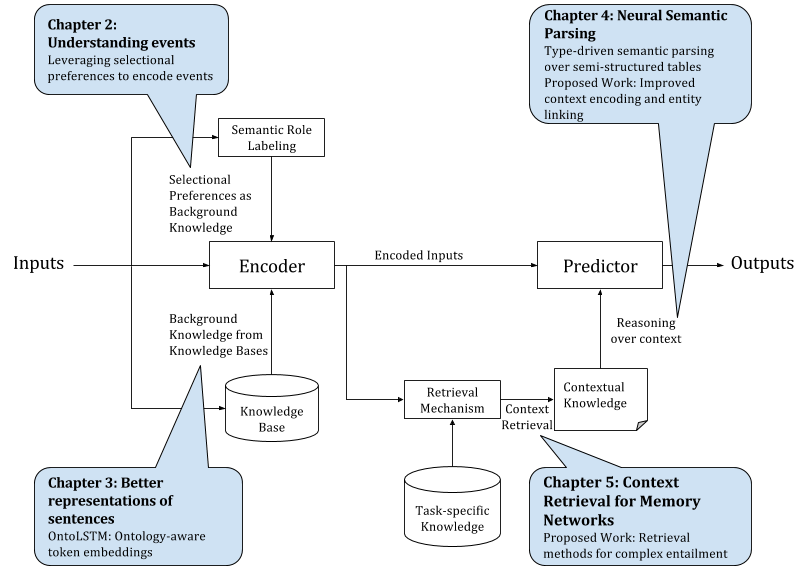
\includegraphics[width=6in]{figures/thesis_overview.png}
\caption{Generic NLU pipeline and thesis overview}
\label{fig:thesis_overview}
\end{center}
\end{figure}
Figure~\ref{fig:thesis_overview} shows the generic pipeline described so far, along with the breakdown of the chapters related to each component
of the pipeline.

In Chapter~\ref{chapter:ontolstm}, we describe a method to incorporate selectional 
preferences in algorithms that encode sentences. This involves a variant of Long Short-Term
Memory (LSTM) based Recurrent Neural Networks (RNN) that use information
from WordNet, a lexical 
ontology. The hybrid model looks at WordNet synsets, and at the hypernym hierarchies of the
words being processed so that the 
encoder is aware of their different senses, and the corresponding type information.
The ontology aware LSTM (OntoLSTM) learns to attend to the appropriate sense,
and the relevant type 
(either the most specific concept or a generalization by choosing a hypernym of
the word), conditioned on the context and the end-objective. We show that the sentence representations 
produced by OntoLSTM are better than those produced by LSTMs when used with identical prediction 
components for predicting textual entailment and preposition phrase attachment. We also visualize the attention scores assigned to the hypernyms 
of words in the input sentences and show that OntoLSTM is indeed learning useful generalizations of words
that help the learned representations perform better at the end task. Proposed work in this chapter is an extension
of the OntoLSTM idea to tree structured encoders that are augmented with subgraph features from a knowledge base. We propose 
to use them to encode open vocabulary semantic parses augmented with information from Freebase.

In Chapter~\ref{chapter:nem} we turn to understanding events.
We describe an annotation effort that resulted in newswire headlines manually labeled with the degree
of surprise associated with them. The NLU task in this chapter is detecting the highly
surprising events as anomalies. This is different from the usual Language Modeling (LM) problem
because even the semantic anomalies are well-formed sentences that can be well-understood. Consequently,
the model needs to discriminate between sentences at a semantic level deeper than surface fluency. Our model encodes events
as a composition of the main verb with its semantic role fillers, and obtains an accuracy of 65\% on the anomaly detection task.
Proposed work in this chapter includes incorporating commonsense knowledge from ConceptNet to improve event representations.

In Chapter~\ref{chapter:memnet_qa} we describe a generalized deep learning architecture for knowledge guided reasoning.
The pipeline follows the generic specification in Section~\ref{sec:intro_external_knowledge} and has configurable components
for encoding and prediction. We identify that the memory network models in \cite{weston2014memory,Sukhbaatar2015EndToEndMN,Xiong2016DynamicMN}
and the attentive reader model from \cite{hermann2015teaching} are specific instantiations of our generic knowledge guided reasoning model.
Unlike prior work that evaluated these models on selecting answers from background text, we evaluate our model on two deep reasoning tasks. The first is
answering science questions, a task that requires a complex entailment model to match the inputs with the context. The second task is
understanding experiment narratives in research papers. Given clauses from a experiment narrative identified as facts, methods,
results, goals and hypotheses, the task is to identify whether the final implications made from the experiment are valid. For this task,
we introduce a dataset of experiments from biomedical research papers annotated by domain experts. This task is similar to the question answering 
task, except that each element in the background knowledge used for reasoning has a specific discourse function.

Finally, in Chapter~\ref{chapter:transfer_learning}, we propose to investigate the transferability of the representations learned for one NLU task to other tasks.
Transfer Learning in neural networks has been well-studied in vision related tasks, and it has been established that the features learned for one task can be
used to improve the performance of similar architectures in other tasks. Within the scope of NLU, this is a feasible investigation given that similarity
among the neural network architectures used for various tasks. It is an important investigation because not all tasks come with lots of training data, owing to factors
such as difficulty in getting reliable annotations and subjectivity. Moreover, with the current trend of increasing model complexity to perform better at any given task,
it is becoming increasingly important to ensure that the models do not overfit any given dataset.